%# -*- coding: utf-8-unix -*-
%%==================================================
%% chapter02.tex for SJTU Master Thesis
%%==================================================

\chapter{SCache的实现}
\label{chap:impl}

本章将展现SCache系统的实现概况。
SCache是一个开源的shuffle数据管理系统,并且提供了一个对于DAG任务预调度的附属调度器。
同时SCache还在设计时提供了跨框架的接口,来实现对于现有主流分布式DAG计算框架的shuffle优化。
在这次实现中,我们以Spark作为DAG计算框架的实例来阐述在SCache辅助下DAG的新的计算流程。
我们首先在章节\ref{sec:overview}中介绍了系统设计的概要。
之后的两个章节主要介绍应用SCache优化上工程上的开销和SCache在容错性上的取舍。

\section{系统设计概要}
\label{sec:overview}

SCache在系统层面上主要包含三个部件:一个分布式的shuffle数据管理系统,一个DAG的附属调度器,和一个Spark系统内部的守护进程。
如图\ref{fig:arch}所示,SCache采用了类似于GFS\cite{gfs}经典的主从节点架构来实现对shuffle数据在集群中的管理。

\begin{figure}[!htp]
	\centering
	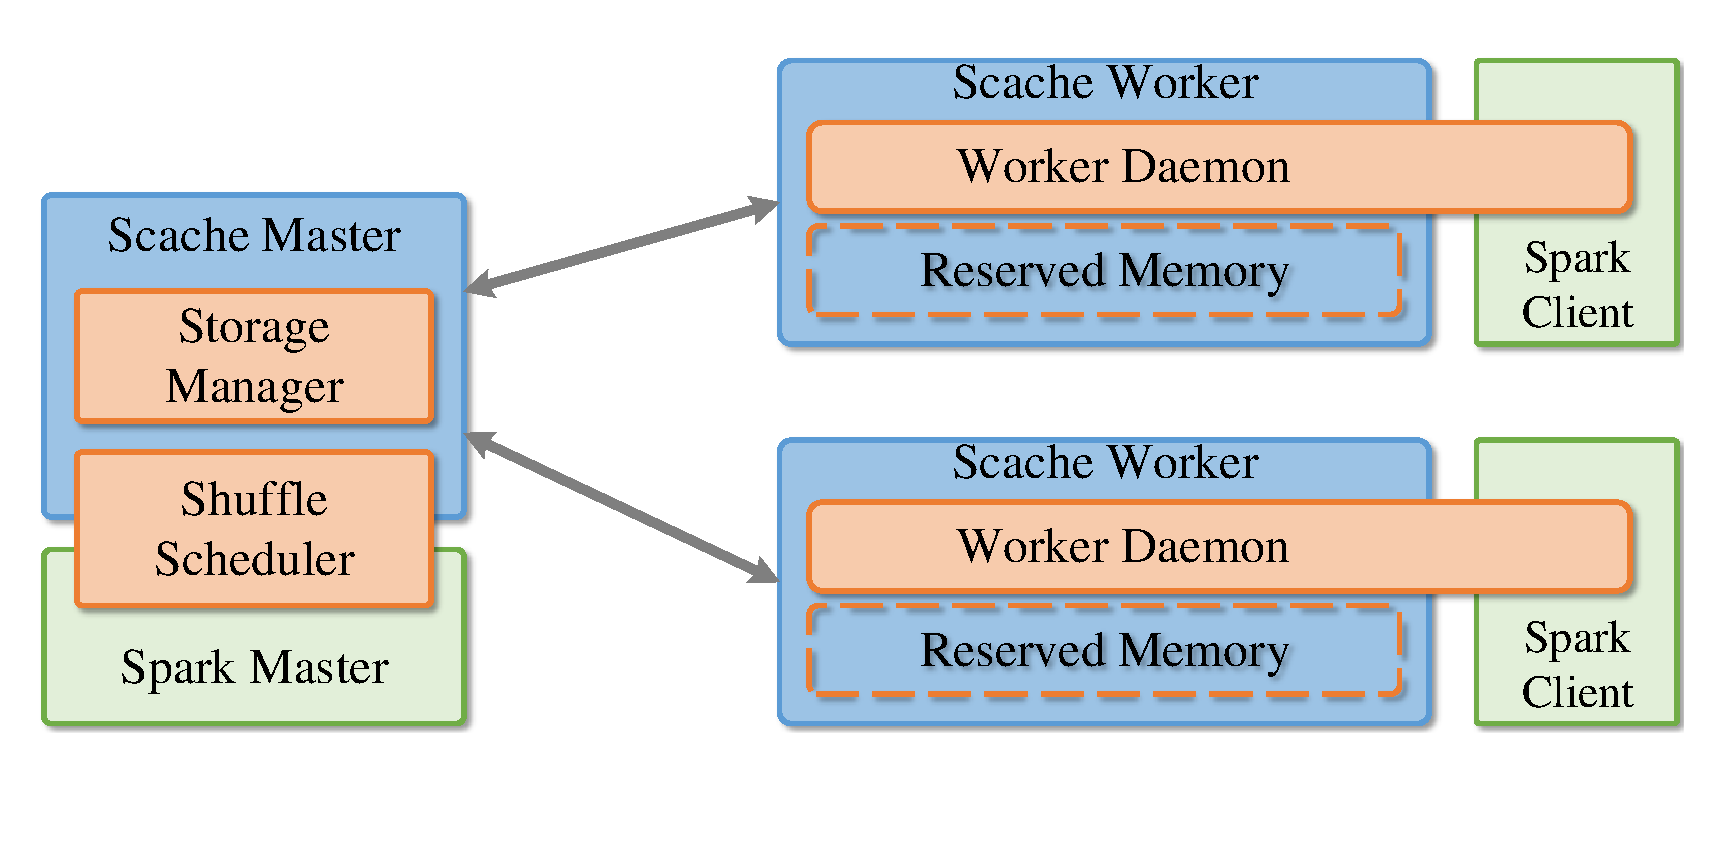
\includegraphics[width=0.6\textwidth]{../../PPoPP-2018/fig/arch.pdf}
	\bicaption[fig:arch]{SCache系统架构示意图}{SCache系统架构示意图}{Fig}{SCache Architecture}
\end{figure}

SCache的主节点负责通过DAG的附属调度器获取Spark上连接shuffle的reduce阶段任务预调度信息,任务的调度执行顺序等。SCache的主节点会根据reduce阶段任务的预调度信息通知到各个从属工作节点。
当工作节点收到任务预调度信息之后,会将本地已经缓存的map任务输出的shuffle数据分别发送到目的节点。
并且对于未完成的map任务,一旦工作节点通过内存拷贝的方式获取了相应的shuffle数据后就立即通过网络将shuffle数据分发出去。
除此之外,SCache主节点还会根据任务的执行顺序信息给各个shuffle的数据单元标注上优先级并且发送给各个工作节点。

SCache的从节点会在本地占用一部分内存空间用来存储shuffle的数据块。
于此同时,当本地的内存空间不够时,各个工作节点会根据从主节点收到的shuffle数据块优先级信息,结合本地的缓存信息(比如是否存在不完整的shuffle存储单元)来将一部分shuffle数据先保存到磁盘上。
本地的工作节点会在内存中至少缓存一个优先级最高的reduce任务需要的shuffle数据。
当本地工作节点的shuffle缓存数据被任务消耗时,该部分内存空间就会被释放,而在磁盘中缓存的较高优先级的数据就会被立刻放入内存中。
通过结合主节点的优先级信息,本地shuffle的缓存状况以及Spark任务对shuffle数据的访问状况,工作节点的调度可以保证相对独立的完成内存管理并且保证:(1)shuffle数据可以在reduce任务开始执行前就被缓存在内存当中并且(2)shuffle数据的内存缓存不会破坏全部或没有以及应用优先级的限制。

SCache中的DAG附属调度器主要负责从Spark的Driver中获取DAG的信息,包括map阶段和reduce阶段中的shuffle数目,map任务的个数和reduce任务的个数以及当前map任务的shuffle输出的数据分别或者采样任务之后的数据分布。
附属调度器会根据以上信息采用相应的线性回归算法或者采样算法来预测shuffle数据的分布,同时调用算法\ref{mhminheap}和算法\ref{hminheap}来作出一个启发式的调度。
在获得最终调度结果之后,附属调度器会将调度结果发送给SCache的主节点。
同时该调度结果也会在Spark任务调度器调度reduce阶段的任务之前将预调度的结果强制到任务调度器上。

守护进程以一个独立的线程的形式存在于Spark的内存空间,通过RPC的方式与SCache进行通信。
并且向Spark系统内部的守护进程则负责向Spark的任务和Driver提供相应的API。

\begin{table}[!hpb]
    \centering
    \bicaption[tab:apis]{SCache编程接口列表}{SCache编程接口列表}{Table}{API list of SCache}
    \begin{tabular}{ | m{2.5cm} | m{8cm} | m{5cm} | }
        \hline
        接口 & 参数 & 作用 \\ [0.5ex]
        \hline
        \hline
        registerShuffles & jobId: Int, shuffleIds: Array[Int], maps: Array[Int], reduces: Array[Int], partitioner: Array[String] & 向SCache注册shuffle \\ \hline
        getBlock & blockId: String & 向SCache获取shuffle的数据块 \\ \hline
        putBlock & blockId: String, data: Array[Byte], len: Int & 向SCache发送shuffle数据块 \\ \hline
        getShuffleStatus & jobId: Int, shuffleId: Int & 向SCache获取reduce任务的预调度结果 \\
        \hline
    \end{tabular}
\end{table}
\section{工作流程}

接下来我们将介绍在SCache的协同下Spark执行DAG的工作流程。
当一个Spark的工作启动时,首先会根据用户的代码生成一个关于RDD(Resilient Distributed Datasets)的系带关系(lineage)。
之后Spark的调度器会从最终的用户RDD递归向前寻找依赖的RDD。
在RDD之间的数据依赖中,如果存在部分依赖,也就是shuffle依赖,Spark会在此处插入一个shuffle过程,并且将之前的所有RDD合并成一个计算阶段(stage)。
递归寻找的过程会在当一个RDD的数据已经被计算或者已经到了存储系统的部分就会停止。
而这些计算阶段则最终组成了计算过程中的DAG逻辑。

对于DAG中相邻计算阶段之间的shuffle依赖,它们会被打包成一个RPC的调用提交到SCache的从属调度器上。如表\ref{apis}中,一个shuffle依赖需要包含一个唯一的整数ID,分区函数的类型,shuffle对应的map阶段任务数以及reduce阶段的任务数。
在收到一次RPC提交之后,SCache的从属调度器会首先检查分区函数的类型,如果不是哈希分区函数,就会通过在Spark的Driver上的守护进程在Spark执行该计算阶段前插入一段采样程序。
我们会在章节\ref{sec:sampling}中详细阐述这个过程。

\section{水塘抽样}
\label{sec:sampling}